\section{Perceptrons multicouches}
\subsection{Données utilisées}
\paragraph{}
Pour cette expérience, j'ai utilisé les données résultant du traitement des images originales et de l'extraction des seuls yeux \ref{data-processing:eyes}.
Le nombre de cas était $\approx500$, les résultats pourraient donc ne pas être très précis.
Je vais relancer cette expérience avec plus de données.
% For this experiment, I used the data resulted from processing the original images and extracting only the eyes \ref{data-processing:eyes}.
% The number of instances was $\approx500$, so the results might not be very accurate.
% I will rerun this experiment with more data.

\subsection{Paramètres d'entraînement}
\paragraph{}
J'ai entraîné ce modèle en utilisant la configuration ci-dessous, pour environ 1000 époques.
J'ai essayé plusieurs optimiseurs, tels que Adam, Adagrad et SGD, mais RMSprop semblait faire les choses très bien.
% I trained this model using the configuration below, for about 1000 epochs.
% I tried multiple optimizers, such as Adam, Adagrad and SGD, but RMSprop seemed to do things just fine.

\begin{lstlisting}[language=python, caption=Formation du MLP]
print('Loading train data...')
X, y = get_data()
X = np.array(X)
y = np.array(y)

print('Training neural network...')
model = Sequential([
    Dense(100, input_shape=(len(X[0]),),
            kernel_initializer='glorot_uniform'),
    Dropout(0.5),
    ReLU(),
    Dense(16, kernel_initializer='glorot_uniform'),
    ReLU(),
    Dense(4, activation='softmax')
])
rmsprop = RMSprop(lr=0.001)
model.compile(optimizer='adagrad',
                loss='categorical_crossentropy', metrics=['accuracy'])
start_time = time.time()
fit_history = model.fit(X, y, epochs=train_parameters["epochs"], verbose=1)
end_time = time.time()
print('Training done')
\end{lstlisting}

\subsection{Résultats}
\paragraph{}
Les tests effectués sur les mêmes données de formation ont donné une précision de plus de $95\%$.
Je vais réexaminer le score des mesures sur des données de test distinctes, après en avoir acquis d'autres.
Cependant, j'ai essayé de prédire où l'utilisateur regarde sur une grille de 2x2 et cela a donné de bons résultats dans l'ensemble.
Bien que ce ne soit pas parfait, il a fait le travail.
% Testing this on the same training data gave an accuracy of over $95\%$.
% I will rerun the metrics score on some separate testing data, after I will have acquired more.
% However, I tried predicting where the user is looking on a 2x2 grid and it did mostly well.
% While it wasn't perfect, it did the job.

\begin{figure}[h]
    \centering
    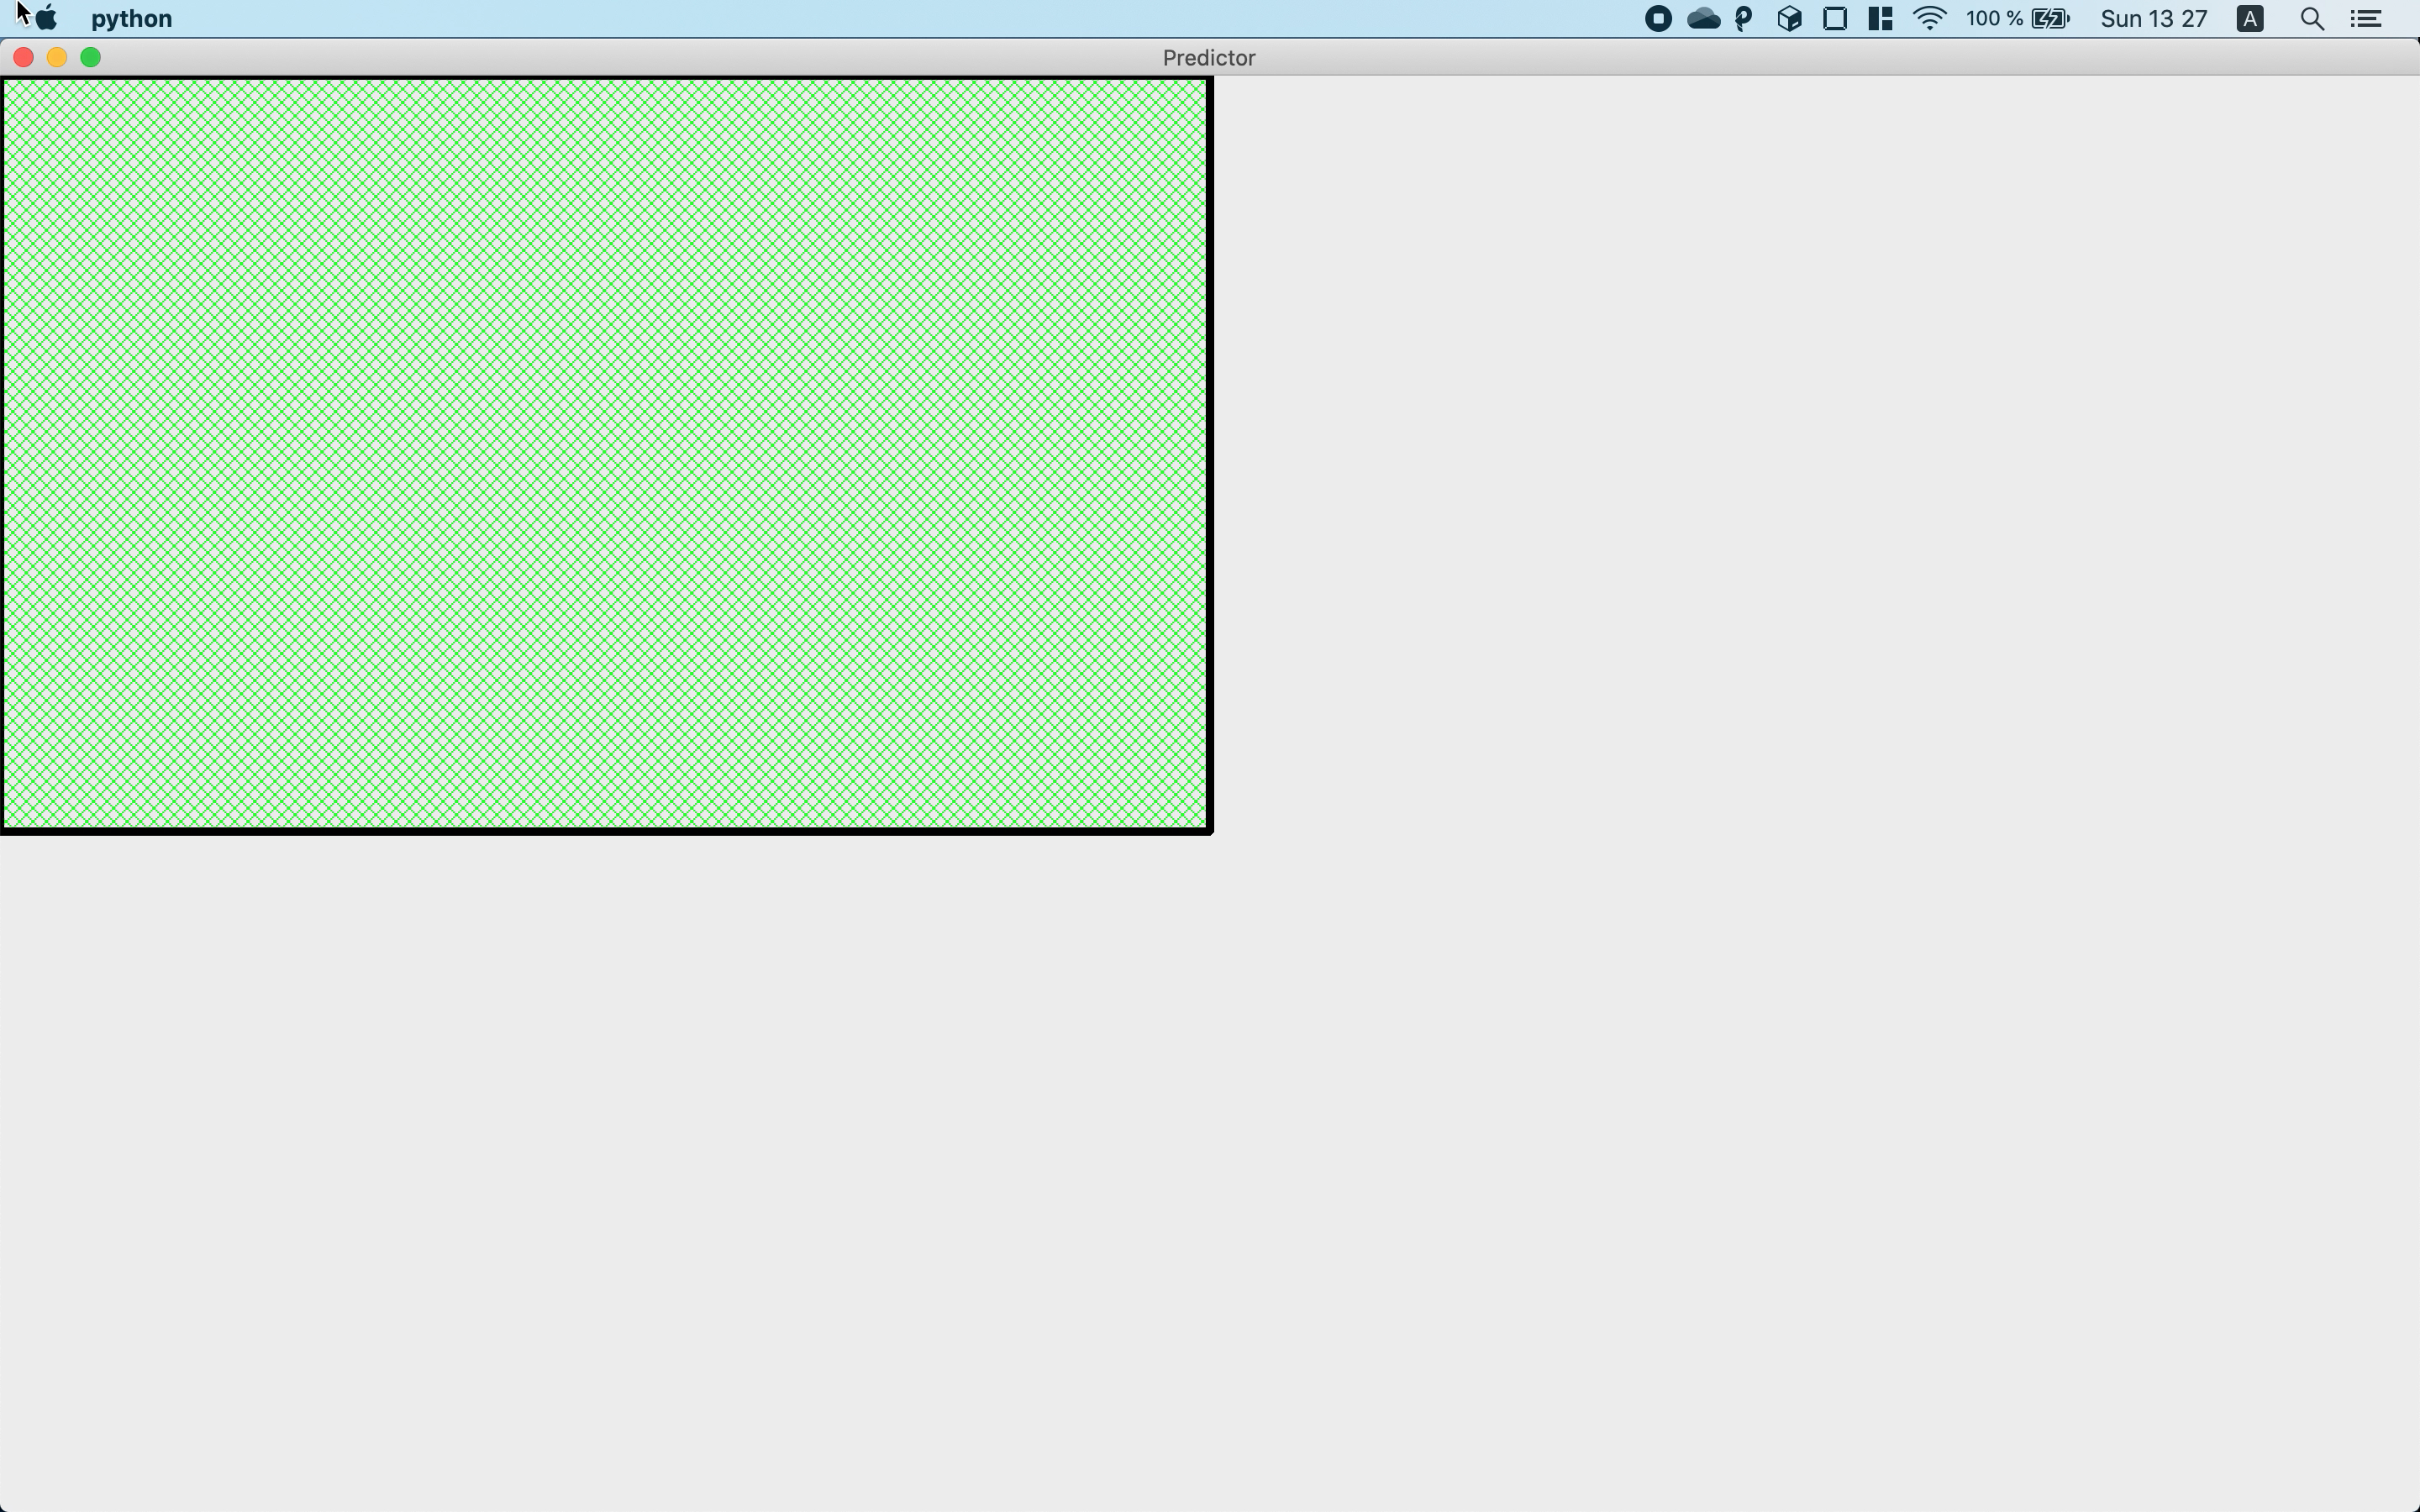
\includegraphics[width=\textwidth]{mlp_prediction.png}
    \caption{Prévision sur une grille 2x2 avec MLP\\En fait, je vraiment regardais dans la partie supérieure gauche de l'écran, croyez-moi!}
    \label{}
\end{figure}

\section{Réseaux neuronaux convolutifs}
\paragraph{}
Il s'agit actuellement d'un travail en cours.
% This is currently a work in progress.